\documentclass[12pt,a4paper]{book}
%\documentclass[a4paper,french]{book}
%\usepackage[17pt]{extsizes}


\input{../1ere-preambule}

\rhead{\textcolor{red}{Correction - DS n$^{\circ}04$ - Dérivation - 14/04/2025}}

\newcommand{\va}[1]{\lvert \ #1 \ \rvert}
\newcommand{\vaf}[1]{\left\lvert \ #1\  \right\rvert}

\begin{document}
	\graphicspath{{images/}}
	
	\begin{center}
		
		
		\fbox{
			\begin{minipage}[]{15cm}
				\begin{center}
					\LARGE{\rule{0.5cm}{0pt}\rule[-0.25cm]{0pt}{0.9cm}
						\textcolor{red}{DS n$^{\circ}04$ - 14/04/2025 \\
						Correction - Dérivation} 
					}
				\end{center}
			\end{minipage}
		}
	\end{center}
	
%	\begin{center}\textbf{1h20min - Barème indicatif}\end{center}
%	\begin{center}\textbf{Les élèves avec un tier-temps ne traitent pas les questions avec  le symbole \ding{46}}\end{center}
%	\begin{center}\textbf{Calculatrice autorisée.\\Les résultats devront être justifiés (à l'aide de calcul ou de propriétés).}\end{center}

\exerciceDS{ - (1,5 points)}

\begin{minipage}[c]{0.48\linewidth}
	A l'aide du graphique ci-contre et sachant que la courbe verte est la courbe représentative de la fonction f et que les droites rouges sont les tangentes à la courbe en 2 ; 4 et 8; déterminer $f'(2)$, $f'(4)$ et $f'(8)$.
	\begin{corrBox}
		$f'(2)=-1$\quad \quad $f'(4)=0$\quad \quad $f'(8)=2$		
	\end{corrBox}
\end{minipage} \hfill
\begin{minipage}[c]{0.48\linewidth}
	\begin{center}
		\newrgbcolor{qqwuqq}{0. 0.39215686274509803 0.}
		\psset{xunit=0.8cm,yunit=0.8cm,algebraic=true,dimen=middle,dotstyle=o,dotsize=5pt 0,linewidth=1.5pt,arrowsize=3pt 2,arrowinset=0.25}
		\begin{pspicture*}(-0.7,-9.2)(9.,0.5)
%			\multips(0,-5)(0,1.0){11}{\psline[linestyle=dashed,linecap=1,dash=1.5pt 1.5pt,linewidth=0.4pt,linecolor=lightgray]{c-c}(-2.5,0)(7.,0)}
%			\multips(-2,0)(1.0,0){10}{\psline[linestyle=dashed,linecap=1,dash=1.5pt 1.5pt,linewidth=0.4pt,linecolor=lightgray]{c-c}(0,-5.)(0,5.2)}
			\psgrid[subgriddiv=0,gridcolor=gray, gridlabels=0pt](-2,-9)(9,1)
			\psaxes[labelFontSize=\scriptstyle,xAxis=true,yAxis=true,Dx=1.,Dy=1.,ticksize=-2pt 0,subticks=2]{->}(0,0)(-2.5,-9.)(9.,0.5)
			\psplot[linewidth=1.2pt,linecolor=qqwuqq,plotpoints=200]{-2.5}{9.0}{0.25*x^(2.0)-2.0*x-2.0}
			\psplot[linewidth=1.2pt,linecolor=red]{-2.5}{9.}{(-3.-1.*x)/1.}
			\psplot[linewidth=1.2pt,linecolor=red]{-2.5}{9.}{(-6.-0.*x)/1.}
			\psplot[linewidth=1.2pt,linecolor=red]{-2.5}{9.}{(-18.--2.*x)/1.}
			%		\begin{scriptsize}
				\rput[bl](-3.52,-11.04){\qqwuqq{$f$}}
				\rput[bl](2.22,5.82){\red{$g$}}
				\rput[bl](-4.14,3.68){\red{$h$}}
				\rput[bl](3.62,5.82){\red{$i$}}
				%		\end{scriptsize}
		\end{pspicture*}
	\end{center}
\end{minipage}





\exerciceDS{ - (2 points)}

\begin{minipage}[c]{0.48\linewidth}
	Dans le graphique ci-contre, tracer les tangentes en 1 et en 3 à la courbe représentative de la fonction f sachant que $f'(1)=2$ et $f'(3)=-6$
\end{minipage} \hfill
\begin{minipage}[c]{0.48\linewidth}
	\begin{center}
		\psset{xunit=0.8cm,yunit=0.8cm,algebraic=true,dimen=middle,dotstyle=o,dotsize=5pt 0,linewidth=1.2pt,arrowsize=3pt 2,arrowinset=0.25}
		\begin{pspicture*}(-2.,-2)(5.,6)
			\psgrid[subgriddiv=0,gridcolor=gray, gridlabels=0pt](-2.,-2)(5.,6)
%			\multips(0,-3)(0,1.0){9}{\psline[linestyle=dashed,linecap=1,dash=1.5pt 1.5pt,linewidth=0.4pt,linecolor=lightgray]{c-c}(-2.,0)(5.,0)}
%			\multips(-2,0)(1.0,0){8}{\psline[linestyle=dashed,linecap=1,dash=1.5pt 1.5pt,linewidth=0.4pt,linecolor=lightgray]{c-c}(0,-3.5)(0,4.5)}
			\psaxes[labelFontSize=\scriptstyle,xAxis=true,yAxis=true,Dx=1.,Dy=1.,ticksize=-2pt 0,subticks=2]{->}(0,0)(-2.,-2)(5.,6)
			\psplot[linewidth=1.2pt,linecolor=ForestGreen,plotpoints=200]{-2.0}{5.0}{-2.0*x^(2.0)+6.0*x}
			\psplot[linewidth=1.2pt,linecolor=red]{-2.0}{5.0}{2*x+2}
			\psplot[linewidth=1.2pt,linecolor=red]{-2.0}{5.0}{-6*x+18}
		\end{pspicture*}
	\end{center}
\end{minipage}

\newpage

\exerciceDS{ - (4 points)}

Déterminer sur $\mathbb{R}$ l'expression de la fonction dérivée de chacune des fonctions suivantes.
\begin{enumMet}
	\item $f(x)= 3x^2-7 x+4$ \quad \corr{$f'(x)=3\times 2x-7=6x-7$} 
	\item $g(x)= 7 x^3+4 x^2-7$ \quad \corr{$g'(x)=7\times 3x^2+4\times 2x-0=21x^2+8x$}
	\item $h(x)= -4x^3+6x^2-3x+2$ \quad \corr{$h'(x)=-4\times 3x^2+6\times 2x-3=-12x^2+12x-3$}
	\item $k(x)=-6 x^3+7 x-5x^2+3$ \quad \corr{$k'(x)=-6\times 3x^2+7-5\times 2x=-18x^2-10x+7	$}
\end{enumMet}

\exerciceDS{ - (4 points)}

Déterminer sur $\mathbb{R}$ l'expression de la fonction dérivée de chacune des fonctions suivantes.
\begin{enumMet}
	\item $f(x)= 0,9 x^2-7,2 x+4$ \quad \corr{$f'(x)=0,9\times 2x-7,2=1,8x-7,2$} 
	\item $g(x)= 3-6 x^2$ \quad \corr{$g'(x)=0-6\times 2x=-12x$} 
	\item $h(x)= 5 x^3-13 x-15$ \quad \corr{$h'(x)=5\times 3x^2-13-0=15x^2-13$} 
	\item $k(x)=-\dfrac{5}{3} x^3-\dfrac{7}{2} x^2$ \quad \corr{$k'(x)=-\dfrac{5}{3}\times 3x^2-\dfrac{7}{2}\times 2x=-5x^2-7x$} 
\end{enumMet}

\exerciceDS{ - (4 points)}

Soit $f$ la fonction définie sur \R par $f(x)=-2x^2+5x-4$
\begin{enumMet}
	\item Déterminer $f'$ la fonction dérivée de $f$ sur \R
	\begin{corrBox}
		$f'(x)=-2\times 2x+5=-4x+5$		
	\end{corrBox}
	\item Etudier le signe de $f'(x)$ sur \R et en déduire les variations de la fonction $f$ sur \R
	\begin{corrBox}
		On commence par résoudre l'équation $f^{\prime}(x)=0$.\\
		Soit : $-4x+5=0$
		
		$$
		\begin{aligned}
			 -4x+5&=0 \\
			 x&=\dfrac{5}{4}
		\end{aligned}
		$$
		
		La fonction $f^{\prime}$ est une fonction affine représentée par une droite dont le coefficient directeur $-4$ est négatif.\\
		Donc $f^{\prime}$ est décroissante. Elle est donc d'abord positive (avant $x=\dfrac{5}{4}$ )\\
		puis négative (après $x=\dfrac{5}{4}$ ).
		\item On dresse le tableau de variations en appliquant le théorème :
		\begin{center}
			\begin{tikzpicture}
				\tkzTabInit{$x$ / 1 , $f'(x)$ / 1, $f(x)$ / 1.5}{$-\infty$, $\dfrac{5}{4}$, $+\infty$}
				\tkzTabLine{, +, z, -, }
				\tkzTabVar{-/ , +/ $-\dfrac{7}{8}$, -/ }
			\end{tikzpicture}
		\end{center}
		$$
		f(\dfrac{5}{4})=-2 \times (\dfrac{5}{4})^{2}+5\times \dfrac{5}{4}-4=-\dfrac{7}{8} .
		$$
		
		La fonction $f$ admet un minimum égal à -7 en $x=2$.		
	\end{corrBox}
\end{enumMet}

\exerciceDS{ - (5 points)}

Soit $f$ la fonction définie sur \R par $f(x)=-2x^3+\dfrac{19}{2}x^2-10x+2$
\begin{enumMet}
	\item Déterminer $f'$ la fonction dérivée de $f$ sur \R
	\begin{corrBox}
		$f(x)=-2\times 3x^2+\dfrac{19}{2}\times 2x-10=-6x^2+19x-10$
	\end{corrBox}
	\item Montrer que $f'(x)=(-3x+2)(2x-5)$
	\begin{corrBox}
		$(-3x+2)(2x-5)=-6x^2+15x+4x-10=-6x^2+19x-10=f'(x)$
	\end{corrBox}
	\item Etudier le signe de $f'(x)$ sur \R et en déduire les variations de la fonction $f$ sur \R
	\begin{corrBox}
		On commence par résoudre l'équation $f^{\prime}(x)=0$ :\\
		$(-3x+2)(2x-5)=0$\\
		$-3x+2=0 \quad$ ou $\quad 2x-5=0$\\
		$x=\dfrac{2}{3} \quad x=\dfrac{5}{2}$
		
		La dérivée s'annule en $\dfrac{2}{3}$ et $\dfrac{5}{2}$ .\\
		Comme $a=-6<0$, les branches de la parabole représentant la fonction dérivée sont tournées vers le bas.\\
		La dérivée est donc d'abord négative, puis positive, puis négative.\\
		\begin{center}
			\begin{tikzpicture}
				\tkzTabInit{$x$ / 1 , $f'(x)$ / 1, $f(x)$ / 1.5}{$-\infty$, $\dfrac{2}{3}$,$\dfrac{5}{2}$, $+\infty$}
				\tkzTabLine{, -, z,+,z, -, }
				\tkzTabVar{+/ ,-/$-\dfrac{28}{27}$, +/ $-\dfrac{118}{125}$, -/ }
			\end{tikzpicture}
		\end{center}
		En effet :\\
		$f(\dfrac{2}{3})=-2\times (\dfrac{2}{3})^{3}+\dfrac{19}{2} \times(\dfrac{2}{3})^{2}-10 \times(\dfrac{2}{3})+2=-\dfrac{28}{27}$\\
		$f(\dfrac{4}{5})=-2\times (\dfrac{4}{5})^{3}+\dfrac{19}{2} \times(\dfrac{4}{5})^{2}-10 \times(\dfrac{4}{5})+2=-\dfrac{118}{125}$		
	\end{corrBox}
\end{enumMet}





\end{document}

